\documentclass{article}

% Symbols
\usepackage{amsfonts, amsthm}
\usepackage{upgreek}
\usepackage{physics}
\usepackage{cancel}
\usepackage{amssymb, latexsym, amsmath}
\usepackage{import}
\usepackage[table,xcdraw]{xcolor}

%Algorithms
\usepackage[ruled,lined,linesnumbered,commentsnumbered]{algorithm2e}

%% Identación
\setlength{\parindent}{0cm}

% Código
\newcommand{\code}[1]{\textcolor{white!25!black}{\texttt{#1}}}
\usepackage{listings}

%AMS
\usepackage{amsthm}
\newtheorem{algo-thm}{Algoritmo}

% Graphics
\usepackage{graphicx}
\usepackage{pgf}

% Margins
\addtolength{\voffset}{-1.5cm}
\addtolength{\hoffset}{-1.5cm}
\addtolength{\textwidth}{3cm}
\addtolength{\textheight}{3cm}

%Header-Footer
\usepackage{fancyhdr}
\renewcommand{\headrulewidth}{1pt}

\newcommand{\set}[1]{
  \left\{ #1 \right\}
}

\footskip = 50pt
\renewcommand{\headrulewidth}{1pt}

\pagestyle{fancyplain}

\begin{document}
\title{UNIVERSIDAD NACIONAL AUT\'ONOMA DE M\'EXICO\\ Facultad de Ciencias}
\author{Integrantes:\\
  Diego Angel Rosas Franco\\
  Adri\'an Aguilera Moreno\\
  Marco Antonio Rivera Silva}
\date{}
\maketitle
\begin{center}
  
\includegraphics[scale=0.20]{../Portada/Portada}\\[0.4cm]
  \Large
  \bf{Modelado y programación}
  \normalsize
\end{center}
\newpage
\fancyhead[r]{ Modelado y programación 2022-2}


\section*{\LARGE{Proyecto 01}}

\subsection*{Instrucciones de instalación, compilación y ejecución.}
Se dará por hecho que el usuario sabe moverse en terminal.
\subsubsection*{Requerimientos previos:}
\begin{itemize}
\item[-] Se debe contar con una versión de Java $8$ o superior en su computadora. De preferencia la versión más reciente.
\end{itemize}

\subsubsection*{Ejecución del proyecto:}
\begin{itemize}
\item[-] Si está leyendo esto significa que desempaquetó con éxito el proyecto.
\item[-] Abra su terminal y diríjase a la ruta donde desempaquetó el proyecto.
\item[-] Una vez estando en la ruta
  
  \code{Proyecto01\_NullPointerException},
  
  diríjase a

  \code{Proyecto01\_NullPointerException/src/fciencias/modelado/}
\item[-] Ejecute: “\code{javac CheemsMart.java}”, esto generará los .class del proyecto.
\item[-] Ejecute: “\code{java CheemsMart}”, esto ejecutará el proyecto mostrándole el menú solicitado para el proyecto.
\end{itemize}

\subsubsection*{Ingreso al sistema:}
A continuación se muestra una tabla de usuarios en la base de datos del sistema.
\begin{table}[h]
  \begin{tabular}{|l|l|l|}
  \hline
  \rowcolor[HTML]{C0C0C0} 
  {\color[HTML]{000000} Username}             & {\color[HTML]{000000} Nombre Completo} & {\color[HTML]{000000} Contraseña} \\ \hline
  Ross                                        & Rosa Victoria Villa Padilla            & Zeldaqwerty                       \\ \hline
  arturGod                                    & Arturo Lemus Pablo                     & Password                          \\ \hline
  fulano                                      & Fulano Federico Fernandez Tragedio     & diosEstaAqui123                   \\ \hline
  \rowcolor[HTML]{C0C0C0} 
  Direccion                                   & Número de cuenta bancaria              & País                              \\ \hline
  Calle Olivos 145, Azulejos, Madrid          & 4510467245                             & España                            \\ \hline
  5ta Avenida No 45, Chicago                  & 1234543210                             & Estados Unidos                    \\ \hline
  Calle Chongus 132, Colonia De las Tragedias & 5578551018                             & Mexico                            \\ \hline
  \end{tabular}
  \end{table}\\
  \textit{Como se aprecia, las contraseñas son muy "seguras", excelentes para esta prueba}.\\
  Para poder ingresar al sistema necesitará el Username y la Contraseña. El ingreso es sensible a mayúsculas y minúsculas.
  


\newpage
\subsection*{Justificación de uso de patrones:}
\subsubsection*{Strategy}
Utilizamos Strategy en en la parte de cambiar el idioma debido a que lo resuelve
de una forma conveniente ya que teníamos pensado utilizar State, sin embargo notamos
que a pesar que en ambos tendríamos que modificar el idioma en tiempo de ejecución
había una gran desventaja al usar State, por ejemplo limitar los estados con múltiples
condiciones para evitar que se tuviera más de un estado a la vez, en cambio Strategy
podíamos controlar que en efecto solo tuviera un idioma de una manera mucho más sencilla
y efectiva, además de que sería sumamente sencillo agregar nuevos idiomas en Strategy
que en State.
\subsubsection*{Decorator}
Implementamos el patrón de diseño Decorator en la parte de descuentos, pues los productos
pueden aplicar a uno o más descuentos, incluso del mismo tipo (al menos no hay una restricción
para esto) de manera conveniente en nuestra implementación, donde el \code{Producto} original
sin modificaciones en precios es el centro del decorador.
\subsubsection*{Proxy}
Decidimos implementar Proxy en la parte del Servidor pues en el PDF del proyecto se dice: \textit{Por cuestiones de seguridad, es imperiosamente necesario que la tienda virtual no cargue directamente el catálogo real, pues si llega a presentar vulnerabilidades de seguridad, cualquiera podría cambiarlo}.\\
Pensamos que para solucionar esto sería bueno tener un objeto Proxy Servidor que nos sirviera de intermediarios con el Servidor Real, por ahora esto no se aprovechó al máximo para los Requerimientos del proyecto, pero lo pensamos a la larga, pues seguramente se harían varias peticiones al Servidor, y justo para preservar la seguridad de la tienda y sus datos el objeto intermediario es una mejor opción.\\



\subsection*{Otros patrones que se pudieron usar:}
\subsubsection*{Iterator}
Pensamos que en vez de usar Proxy en el Servidor podríamos usar Iterator, y así regresar un iterador de las estructuras que necesitaramos, sin embargo, a la larga esto podría hacer rigido el sistema, en el sentido de que cuando se quiera agregar seguridad al programa, se debería dar una solución especifica o agregar un nuevo patrón. En cambio con Proxy ya ayudamos a que la seguridad sea mantenible.

\subsubsection*{Singleton}
Nos percatamos que podíamos haber usado Singleton en la clase Servidor, pues de esa forma
tendríamos un servidor centralizado en el que tendríamos a todos nuestros usarios y el catálogo
de la tienda. Sin embargo, vimos que esto podría causar un problema de rigidez, pues a futuro
es posible que la tienda planeé tener servidores a lo largo del mundo para mejorar la velocidad
de respuesta acorde a la región en la que se encuentre el usuario (teoricamente hablando), y
en cada servidor, regional por ejemplo, tener un catálogo distinto a futuro, ya que actualmente
solo se tiene un catálogo en el mismo idioma para todas las regiones. Debido a esto es que
Servidor cuenta con un identificador único, para asi poder diferenciarlo de los demás servidores
futuros.

\subsubsection*{Template}
Pensamos en usar template en los idiomas, de hecho al final se quedó esta idea que tuvimos, la cual fue tener un menuPrincipal() en MenuCompra donde se llamarían ciertos métodos con mensajes al usuario en su idioma, y justo los MenuCompra<Idioma> estarían definiendo estos métodos o "pasos". Pero el problema aqui era que menuPrincipal no era secuencial y debido a eso no se podría aplicar el patrón a menos que lo hicieramos de forma secuenciañ.

\newpage
\subsection*{Diagrama UML:}
\begin{center}
  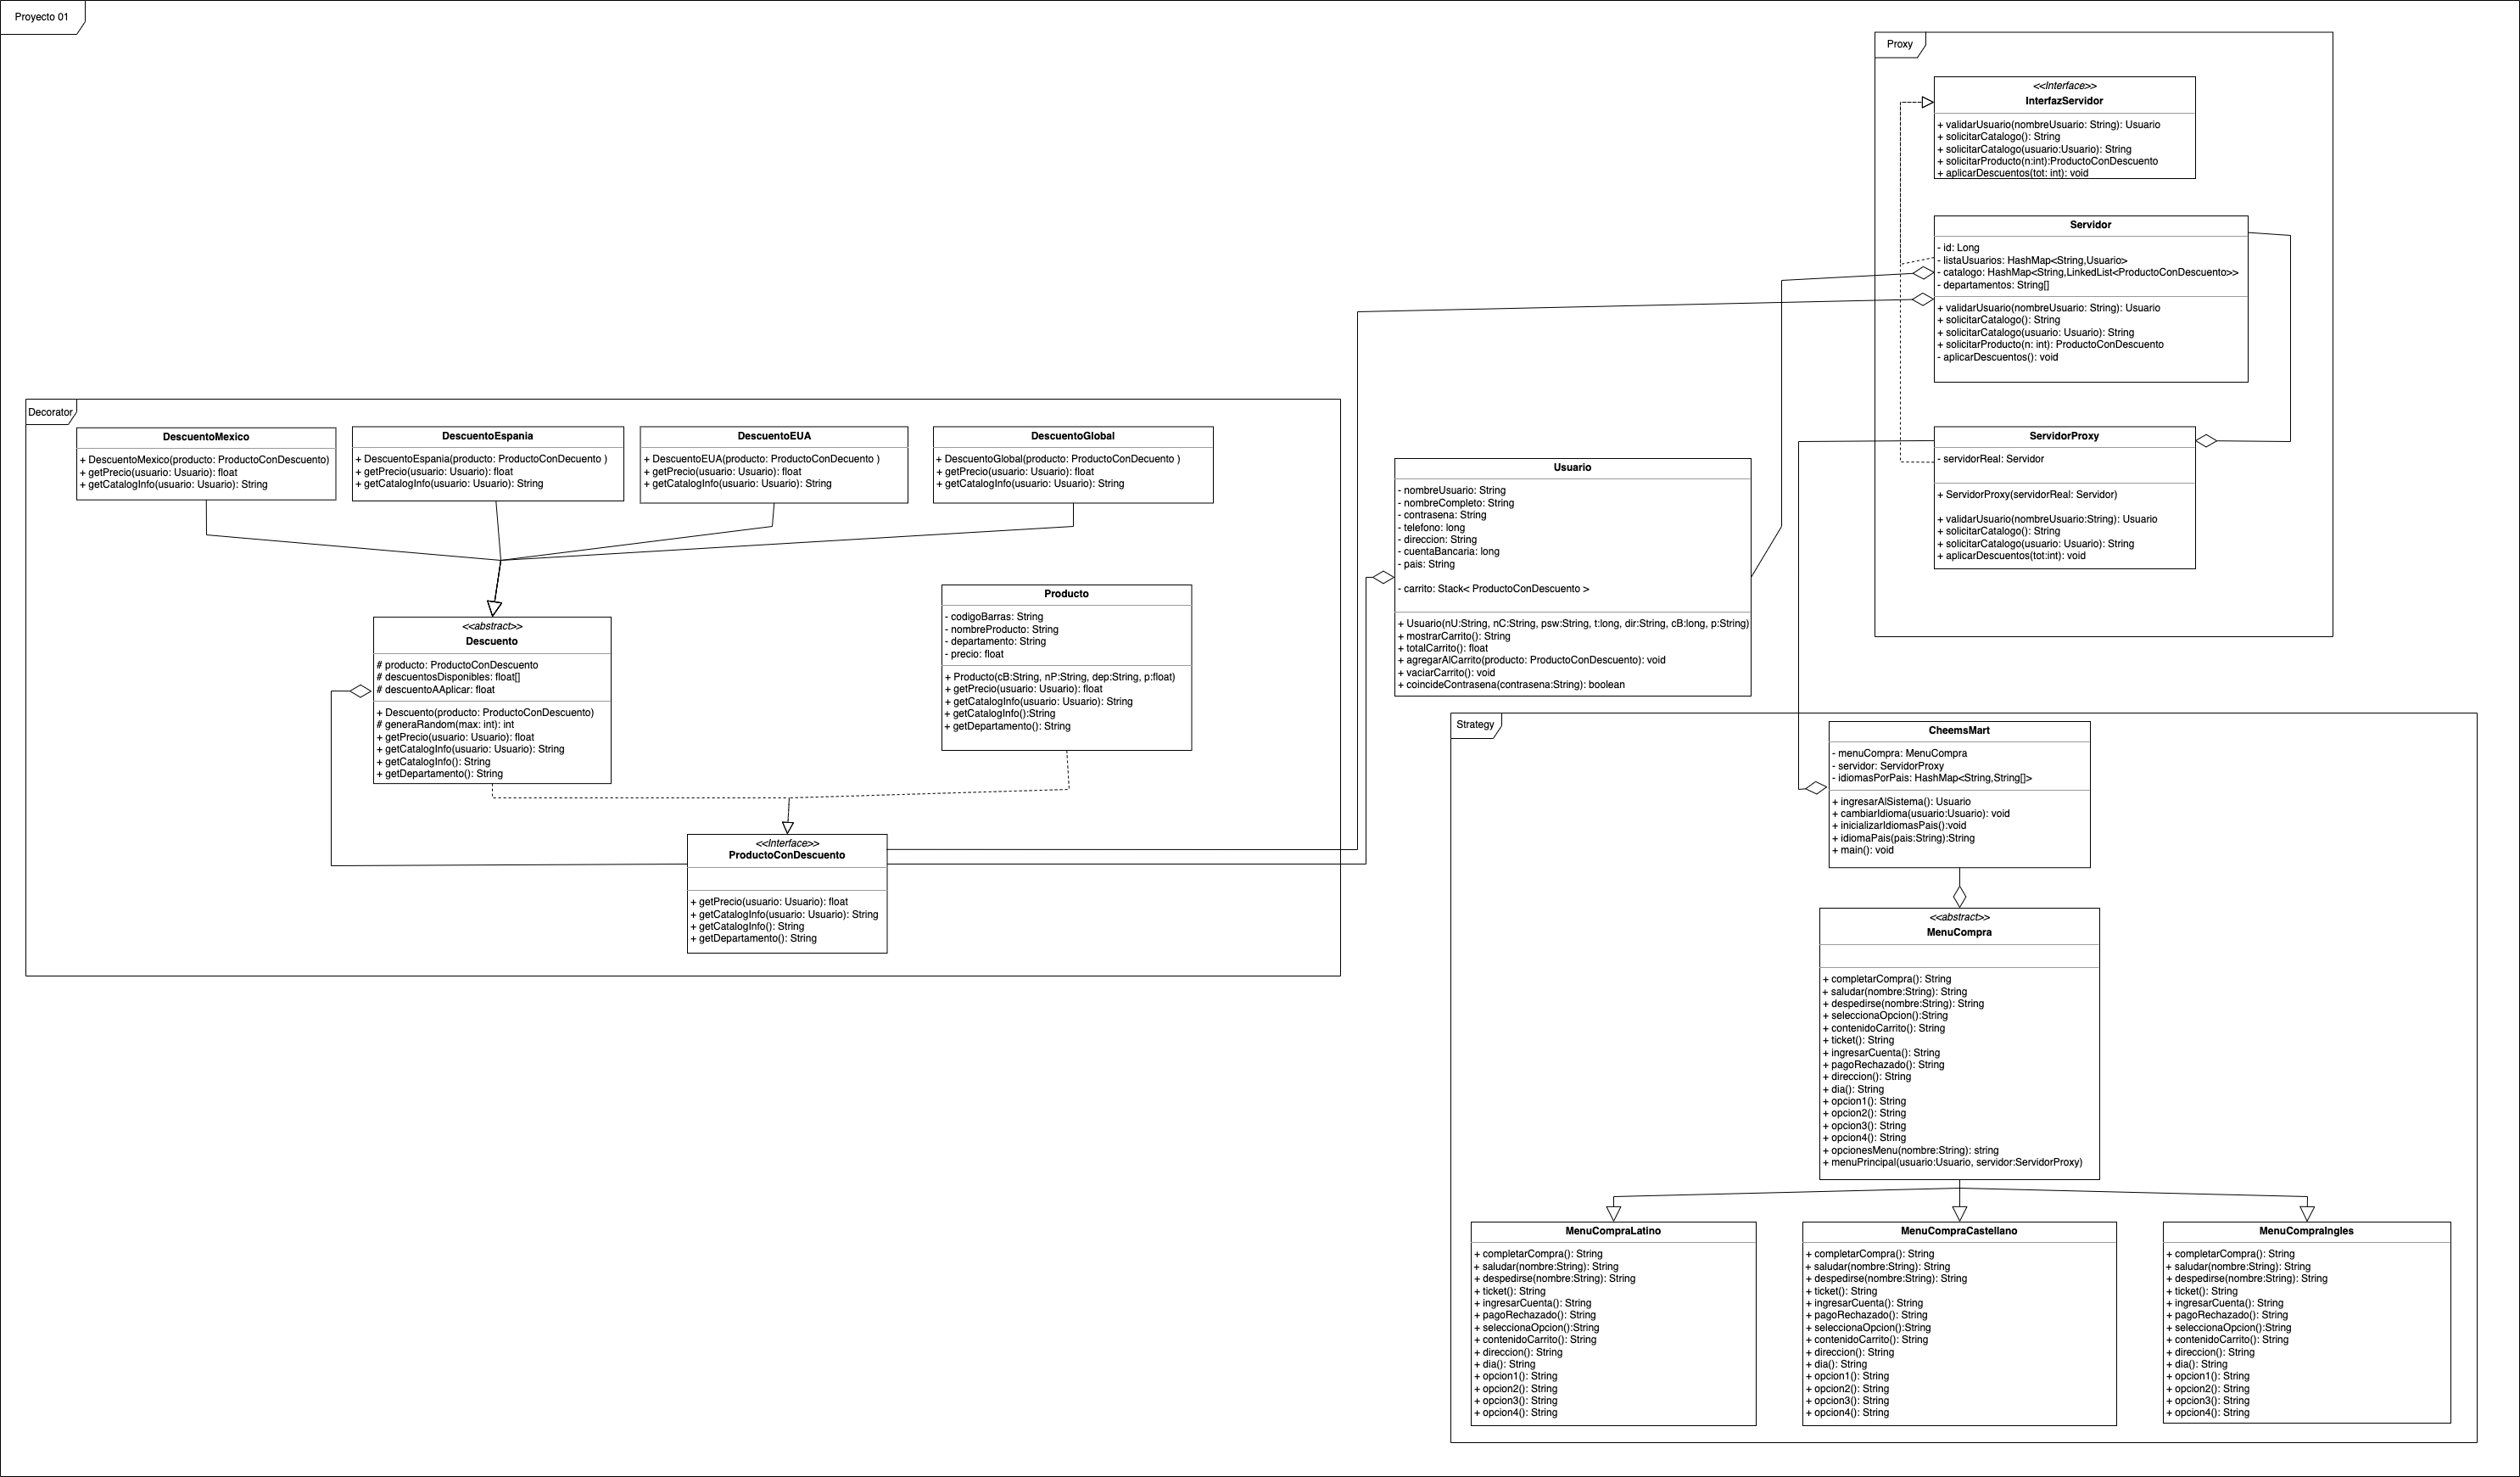
\includegraphics[scale=0.14]{./Proyecto01UML.png}
\end{center}

\subsection*{Diagrama de secuencia:}
\begin{center}
  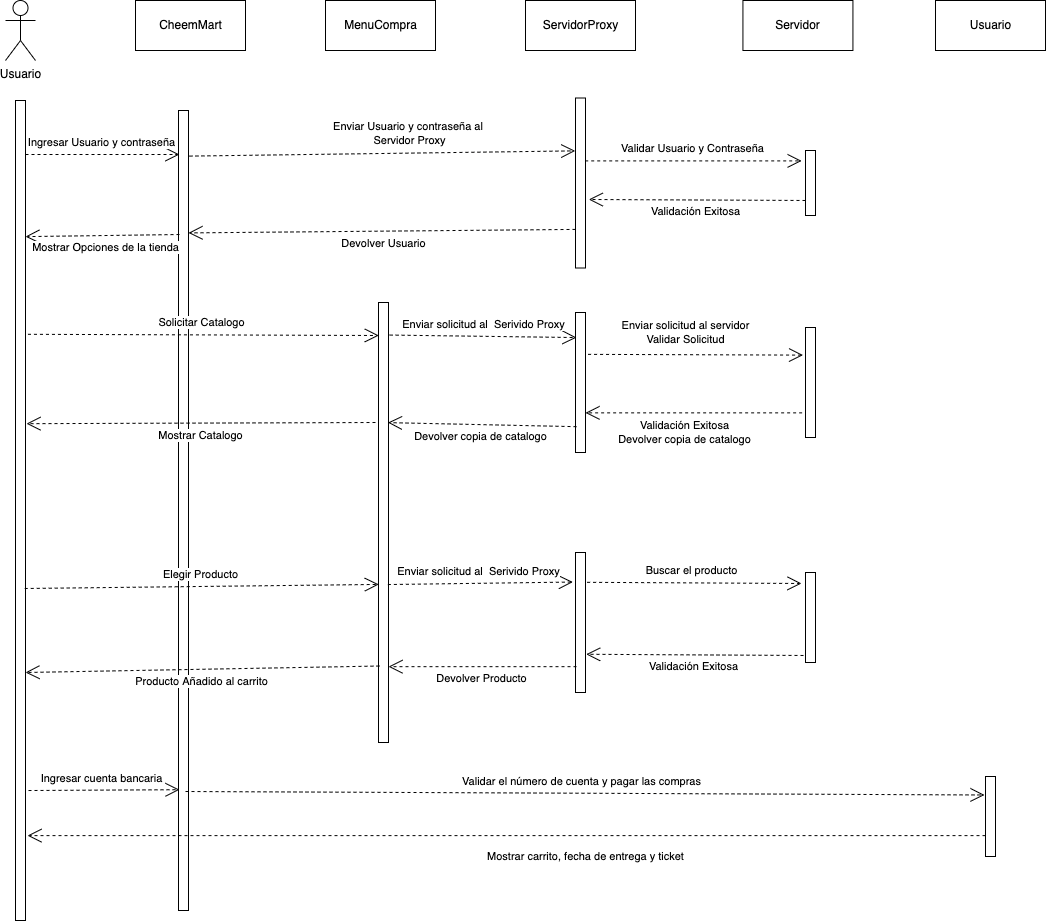
\includegraphics[scale=0.32]{./Proyecto01DiagramaSecuencia.png}
\end{center}
\end{document}
